
\chapter{Error messages and problem resolutions}
\label{chap:error_messages}

All known problems in using the software should be listed and explained in
details using the structure presented below.

Contact information for reporting any problems (either with the software or
this document) should be clearly indicated




\section{VM -Name or/and -Description is empty} 

\subsection{Problem identification}
The faced problem means that the SysAdmin has not specified a name and/or a
description for the virtual machine that he wants to create.

\begin{figure}[H]
\centering
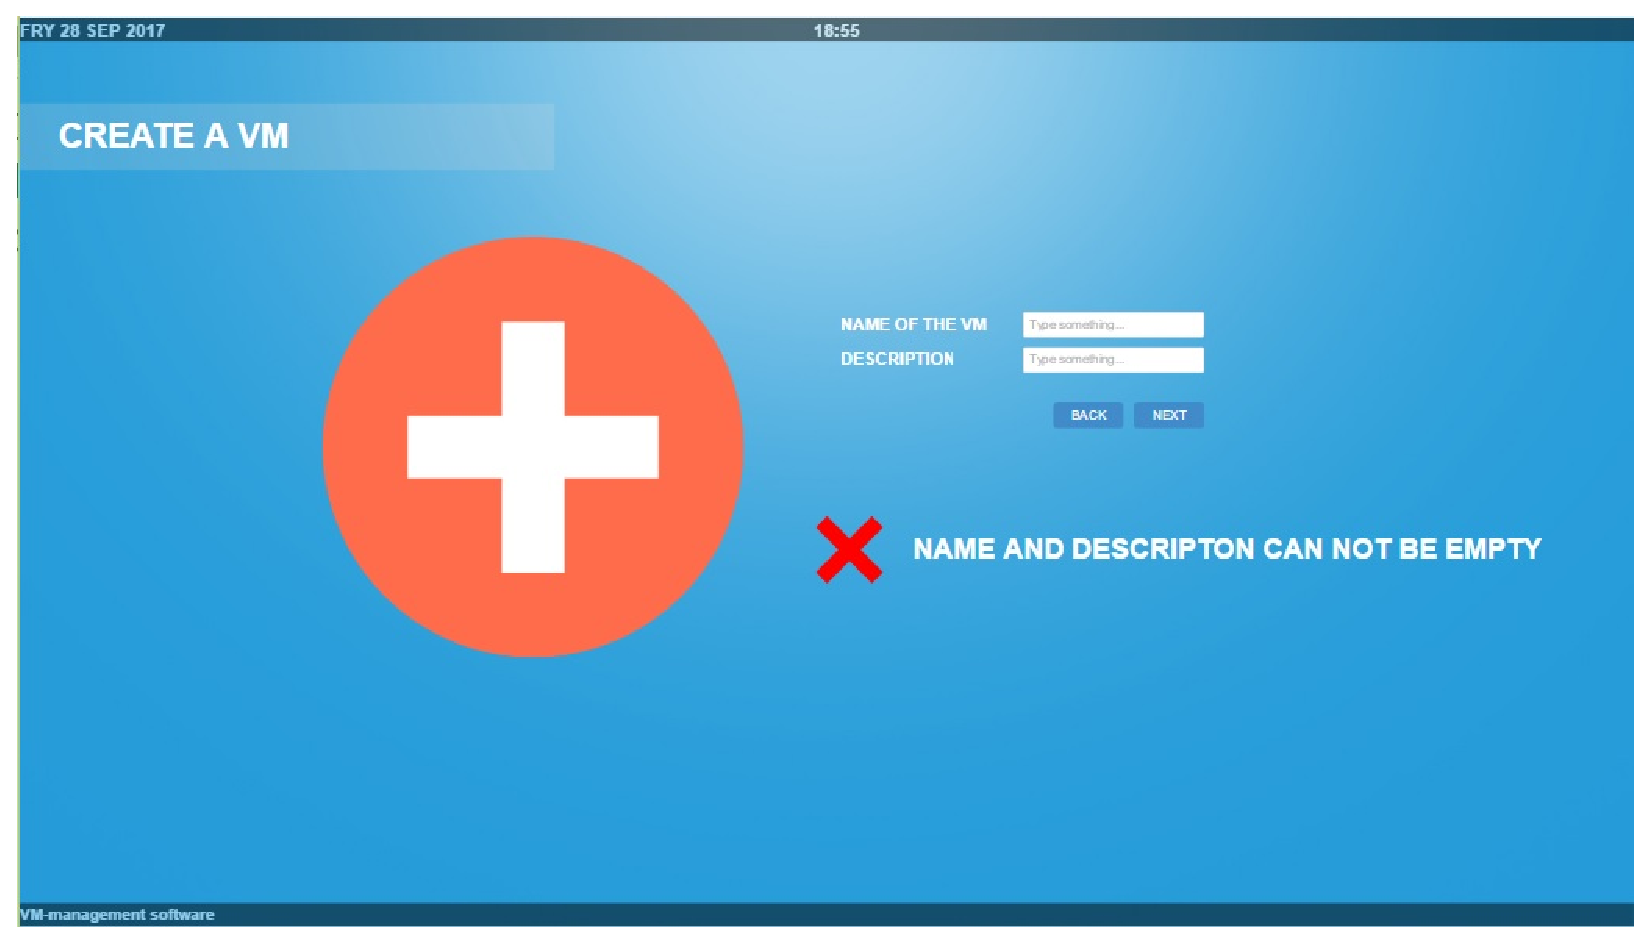
\includegraphics[width=170mm]{images/namedescription.eps}
\caption{\label{overflow}}
\end{figure}

\subsection{Probable cause}

The reason why such a problem has been raised is:\\
\begin{description}
\item[$\bullet$] The SysAdmin has not filled the textfield for the virtual
machine name and/or the textfield representing the description for the virtual
machine.
\end{description}


\subsection{Corrective actions}

A correction for the problem is to:\\
\begin{description}
\item[$\bullet$] The SysAdmin needs to make sure that he filled out both of
the textfields.  More informations about 'How to create a vm' can be found in
section\ldots

\end{description}





\section{Missing Date} 

\subsection{Problem identification}
The faced problem means that the SysAdmin has not selected a date.

\begin{figure}[H]
\centering
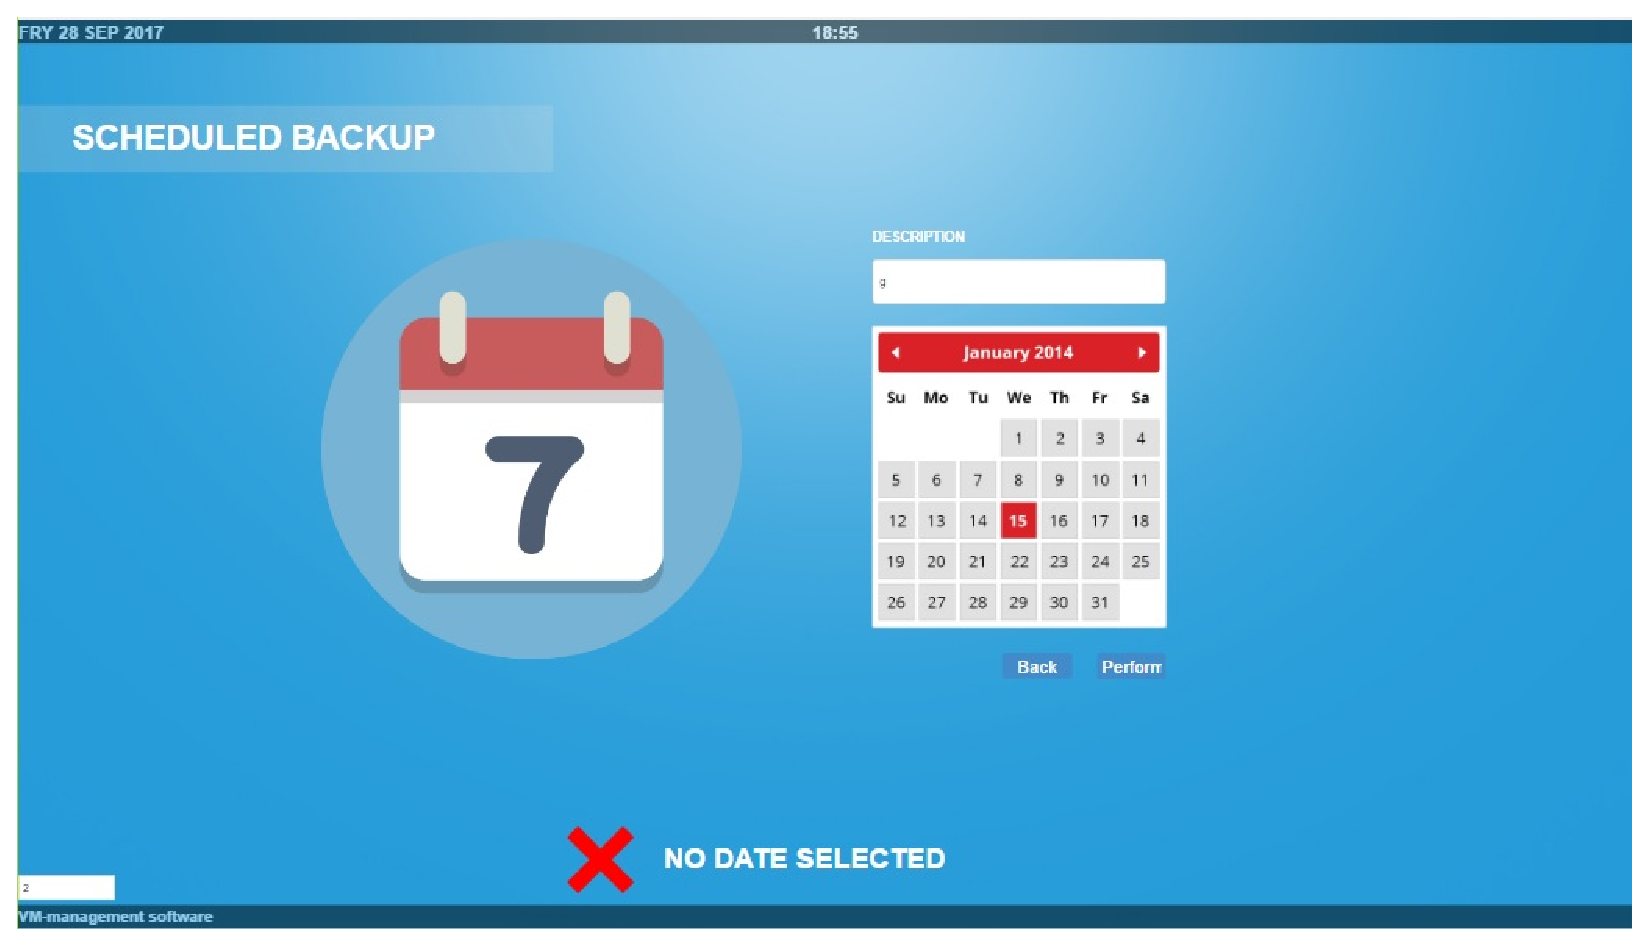
\includegraphics[width=170mm]{images/date.eps}
\caption{\label{overflow}}
\end{figure}

\subsection{Probable cause}

The reason why such a problem has been raised is:\\
\begin{description}
\item[$\bullet$] The date when the backup is going to be performed is missing.
\end{description}


\subsection{Corrective actions}

A correction for the problem is to:\\
\begin{description}
\item[$\bullet$] The SysAdmin needs to make sure that he selected a date before
creating a scheduled backup. More informations about 'How to perform a scheduled
backup' can be found in section\ldots

\end{description}







\section{Missing Backup-Description} 

\subsection{Problem identification}
The faced problem means that the SysAdmin has not provided a description for
the backup.

\begin{figure}[H]
\centering
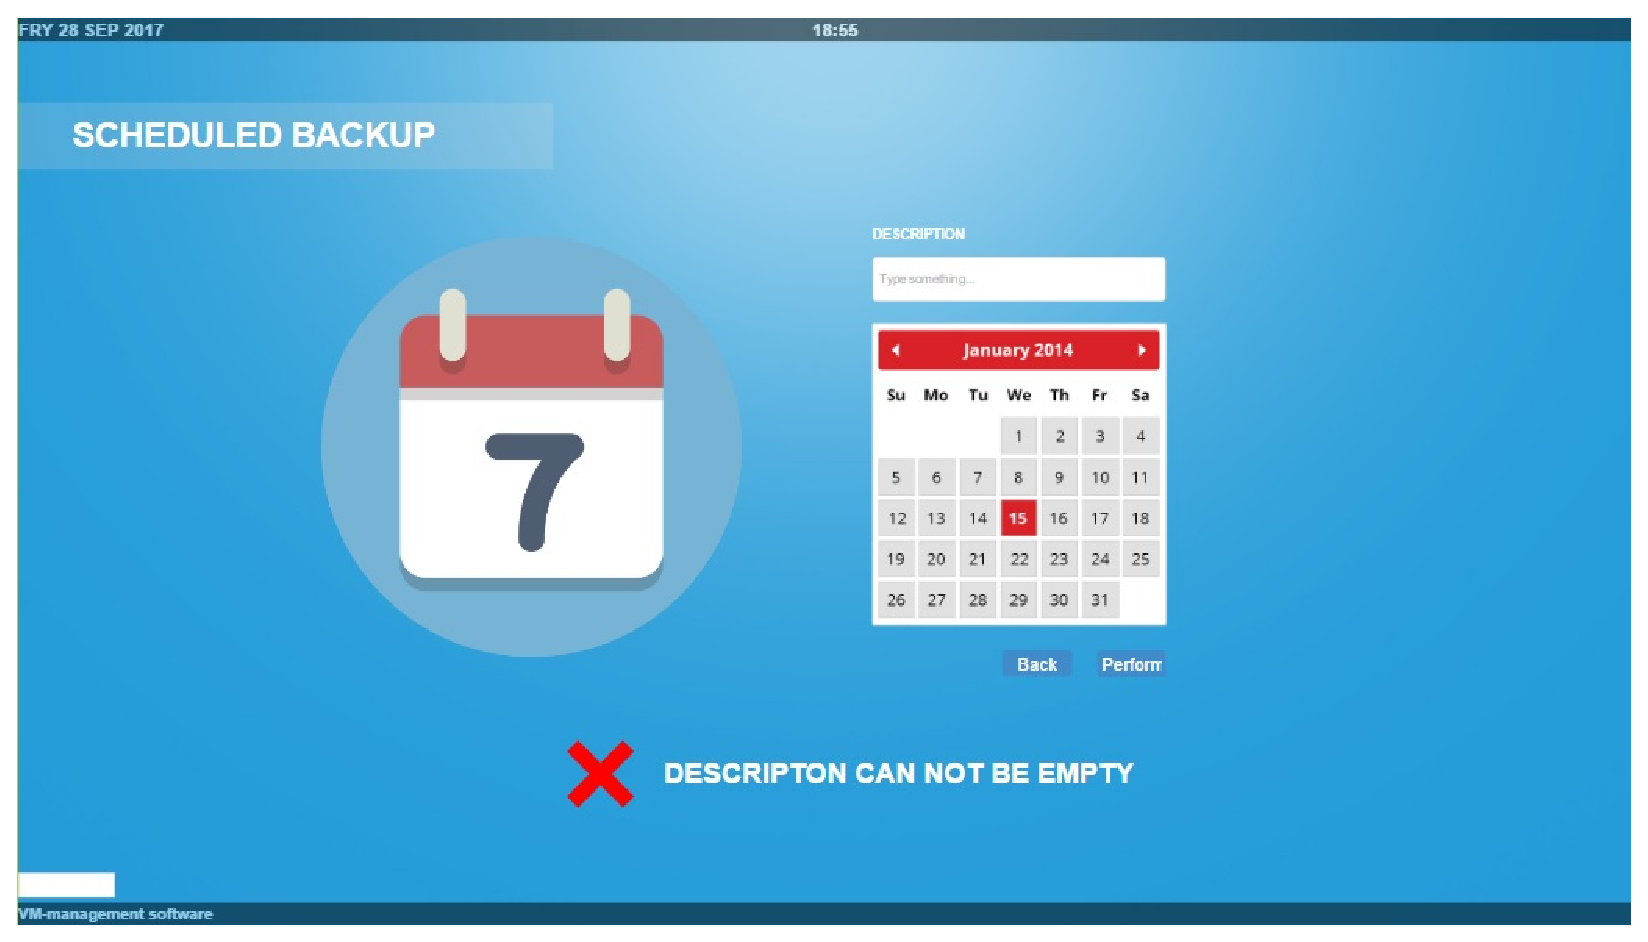
\includegraphics[width=170mm]{images/descriptionback.eps}
\caption{\label{overflow}}
\end{figure}

\subsection{Probable cause}

The reason why such a problem has been raised is:\\
\begin{description}
\item[$\bullet$] The description for the scheduled backup is missing.
\end{description}


\subsection{Corrective actions}

A correction for the problem is to:\\
\begin{description}
\item[$\bullet$] The SysAdmin needs to make sure that textfield for the backup
description is not empty. More informations about 'How to perform a scheduled
backup' can be found in section\ldots

\end{description}










\section{Wrong password deletion canceled} 

\subsection{Problem identification}
The faced problem means that the SysAdmin has not provided the correct password.

\begin{figure}[H]
\centering

\includegraphics[width=170mm]{images/wrongpassword.eps}
\caption{\label{overflow}}
\end{figure}

\subsection{Probable cause}

The reason why such a problem has been raised is:\\
\begin{description}
\item[$\bullet$] The SysAdmin has not typed in the correct password which is
required in order to perform the desired operation.
\end{description}


\subsection{Corrective actions}

A correction for the problem is to:\\
\begin{description}
\item[$\bullet$] The SysAdmin needs to make sure that he provided the correct
password. More informations about 'How to delete a vm' can be found in
section\ldots

\end{description}






\section{Unable to send a component request}

\subsection{Problem identification}
The problem occurs when a SuperSysAdmin cannot send a component request to the
datacenter.

\begin{figure}[H]
\centering
\includegraphics[width=170mm]{images/requestComponent_error.eps}
\caption{\label{overflow}}
\end{figure}

\subsection{Probable cause}

The reason why such a problem has been raised is:\\
\begin{description}
\item[$\bullet$] The SuperSysAdmin has not choosen any components to request.
\end{description}


\subsection{Corrective actions}

A correction for the problem is to:\\
\begin{description}
\item[$\bullet$] The SuperSysAdmin makes sure that he has selected at least a
component model with a quantity.
\end{description}



\section{Missing or Wrong Login information} 

\subsection{Problem identification}
The problem occurs when an actor don't fill the "Password","UserName" textfield
or fills both but with wrong information.

\begin{figure}[H]
\centering
\includegraphics[width=170mm]{images/Login error.eps}
\caption{\label{overflow}}
\end{figure}


\subsection{Probable cause}

The reason why such a problem has been raised is:\\
\begin{description}
\item[$\bullet$] A value in the ''Password'' textfield is missing.
\item[$\bullet$] A value in the ''UserName'' textfield is missing.
\item[$\bullet$] A value in the ''Password'' textfield is wrong.
\item[$\bullet$] A value in the ''UserName'' textfield is wrong.
\end{description}


\subsection{Corrective actions}

A correction for the problem is to:\\
\begin{description}
\item[$\bullet$] The actor needs to make sure that he fills the
''UserName'' and ''Password'' textfields with values that are considered
valid.\ldots

\end{description}






\section{Missing personal information} 

\subsection{Problem identification}
The problem occurs when a Super-SysAdmin don't fill all the differents
textfields with the appropriate value.

\begin{figure}[H]
\centering
\includegraphics[width=170mm]{images/MissingPersonInfos error.eps}
\caption{\label{overflow}}
\end{figure}
\subsection{Probable cause}

The reason why such a problem has been raised is:\\
\begin{description}
\item[$\bullet$] A value in the ''FirstName'' textfield is missing.
\item[$\bullet$] A value in the ''LastName'' textfield is missing.
\item[$\bullet$] A value in the ''User username'' textfield is missing.
\item[$\bullet$] A value in the ''E-mail'' textfield is missing.
\item[$\bullet$] A value in the ''Create Password'' textfield is missing.
\item[$\bullet$] A value in the ''Confirm Password'' textfield is missing.
\item[$\bullet$] A value in the ''Phone Number'' textfield is missing.

\end{description}


\subsection{Corrective actions}

A correction for the problem is to:\\
\begin{description}
\item[$\bullet$] The Super-SysAdmin needs to make sure that all the textfields
for the personal information are not empty.\ldots

\end{description}


\section{Wrong password} 

\subsection{Problem identification}
The faced problem means that the actor has not provided the correct password.

\begin{figure}[H]
\centering

\includegraphics[width=170mm]{images/wrongpassword.eps}
\caption{\label{overflow}}
\end{figure}
\subsection{Probable cause}

The reason why such a problem has been raised is:\\
\begin{description}
\item[$\bullet$] The actor has not typed the correct password which is
required.
\end{description}


\subsection{Corrective actions}

A correction for the problem is to:\\
\begin{description}
\item[$\bullet$] The actor needs to make sure that he provided the correct
password.\ldots

\end{description}


\section{Missing new password} 

\subsection{Problem identification}
The problem occurs when an actor don't fill the "new password" textfield.

\begin{figure}[H]
\centering
\includegraphics[width=170mm]{images/MissingPw Error.eps}
\caption{\label{overflow}}
\end{figure}
\subsection{Probable cause}

The reason why such a problem has been raised is:\\
\begin{description}
\item[$\bullet$] A value in the ''new password'' textfield is missing.
\end{description}


\subsection{Corrective actions}

A correction for the problem is to:\\
\begin{description}
\item[$\bullet$] The actor needs to make sure that he fills the
''new password'' textfield with a new password.\ldots

\end{description}




\section{Missing new e-mail} 

\subsection{Problem identification}
The problem occurs when an actor don't fill the "new E-mail" textfield.

\begin{figure}[H]
\centering
\includegraphics[width=170mm]{images/MissingEmail eror.eps}
\caption{\label{overflow}}
\end{figure}

\subsection{Probable cause}

The reason why such a problem has been raised is:\\
\begin{description}
\item[$\bullet$] A value in the ''new E-mail'' textfield is missing.
\end{description}


\subsection{Corrective actions}

A correction for the problem is to:\\
\begin{description}
\item[$\bullet$] The actor needs to make sure that he fills the
''new E-mail'' textfield with a new e-mail.\ldots

\end{description}




\section{Missing new id} 

\subsection{Problem identification}
The problem occurs when an actor don't fill the "new ID" textfield.

\begin{figure}[H]
\centering
\includegraphics[width=170mm]{images/MissingId error.eps}
\caption{\label{overflow}}
\end{figure}
\subsection{Probable cause}

The reason why such a problem has been raised is:\\
\begin{description}
\item[$\bullet$] A value in the ''new ID'' textfield is missing.
\end{description}


\subsection{Corrective actions}

A correction for the problem is to:\\
\begin{description}
\item[$\bullet$] The actor needs to make sure that he fills the
''new ID'' textfield with a new id.\ldots

\end{description}












